\section{System Architecture and Methodology}
\label{sec:architecture}

The ZeroEdge-NIDS platform is structured as a modular four-tier architecture designed to execute both uncompressed floating-point and integer-quantized inference graphs under identical mathematical conditions. The layered architecture is illustrated in Fig.~\ref{fig:arch}, while the end-to-end data transformation pipeline is depicted in Fig.~\ref{fig:flow}.

\begin{figure}[t]
\centering
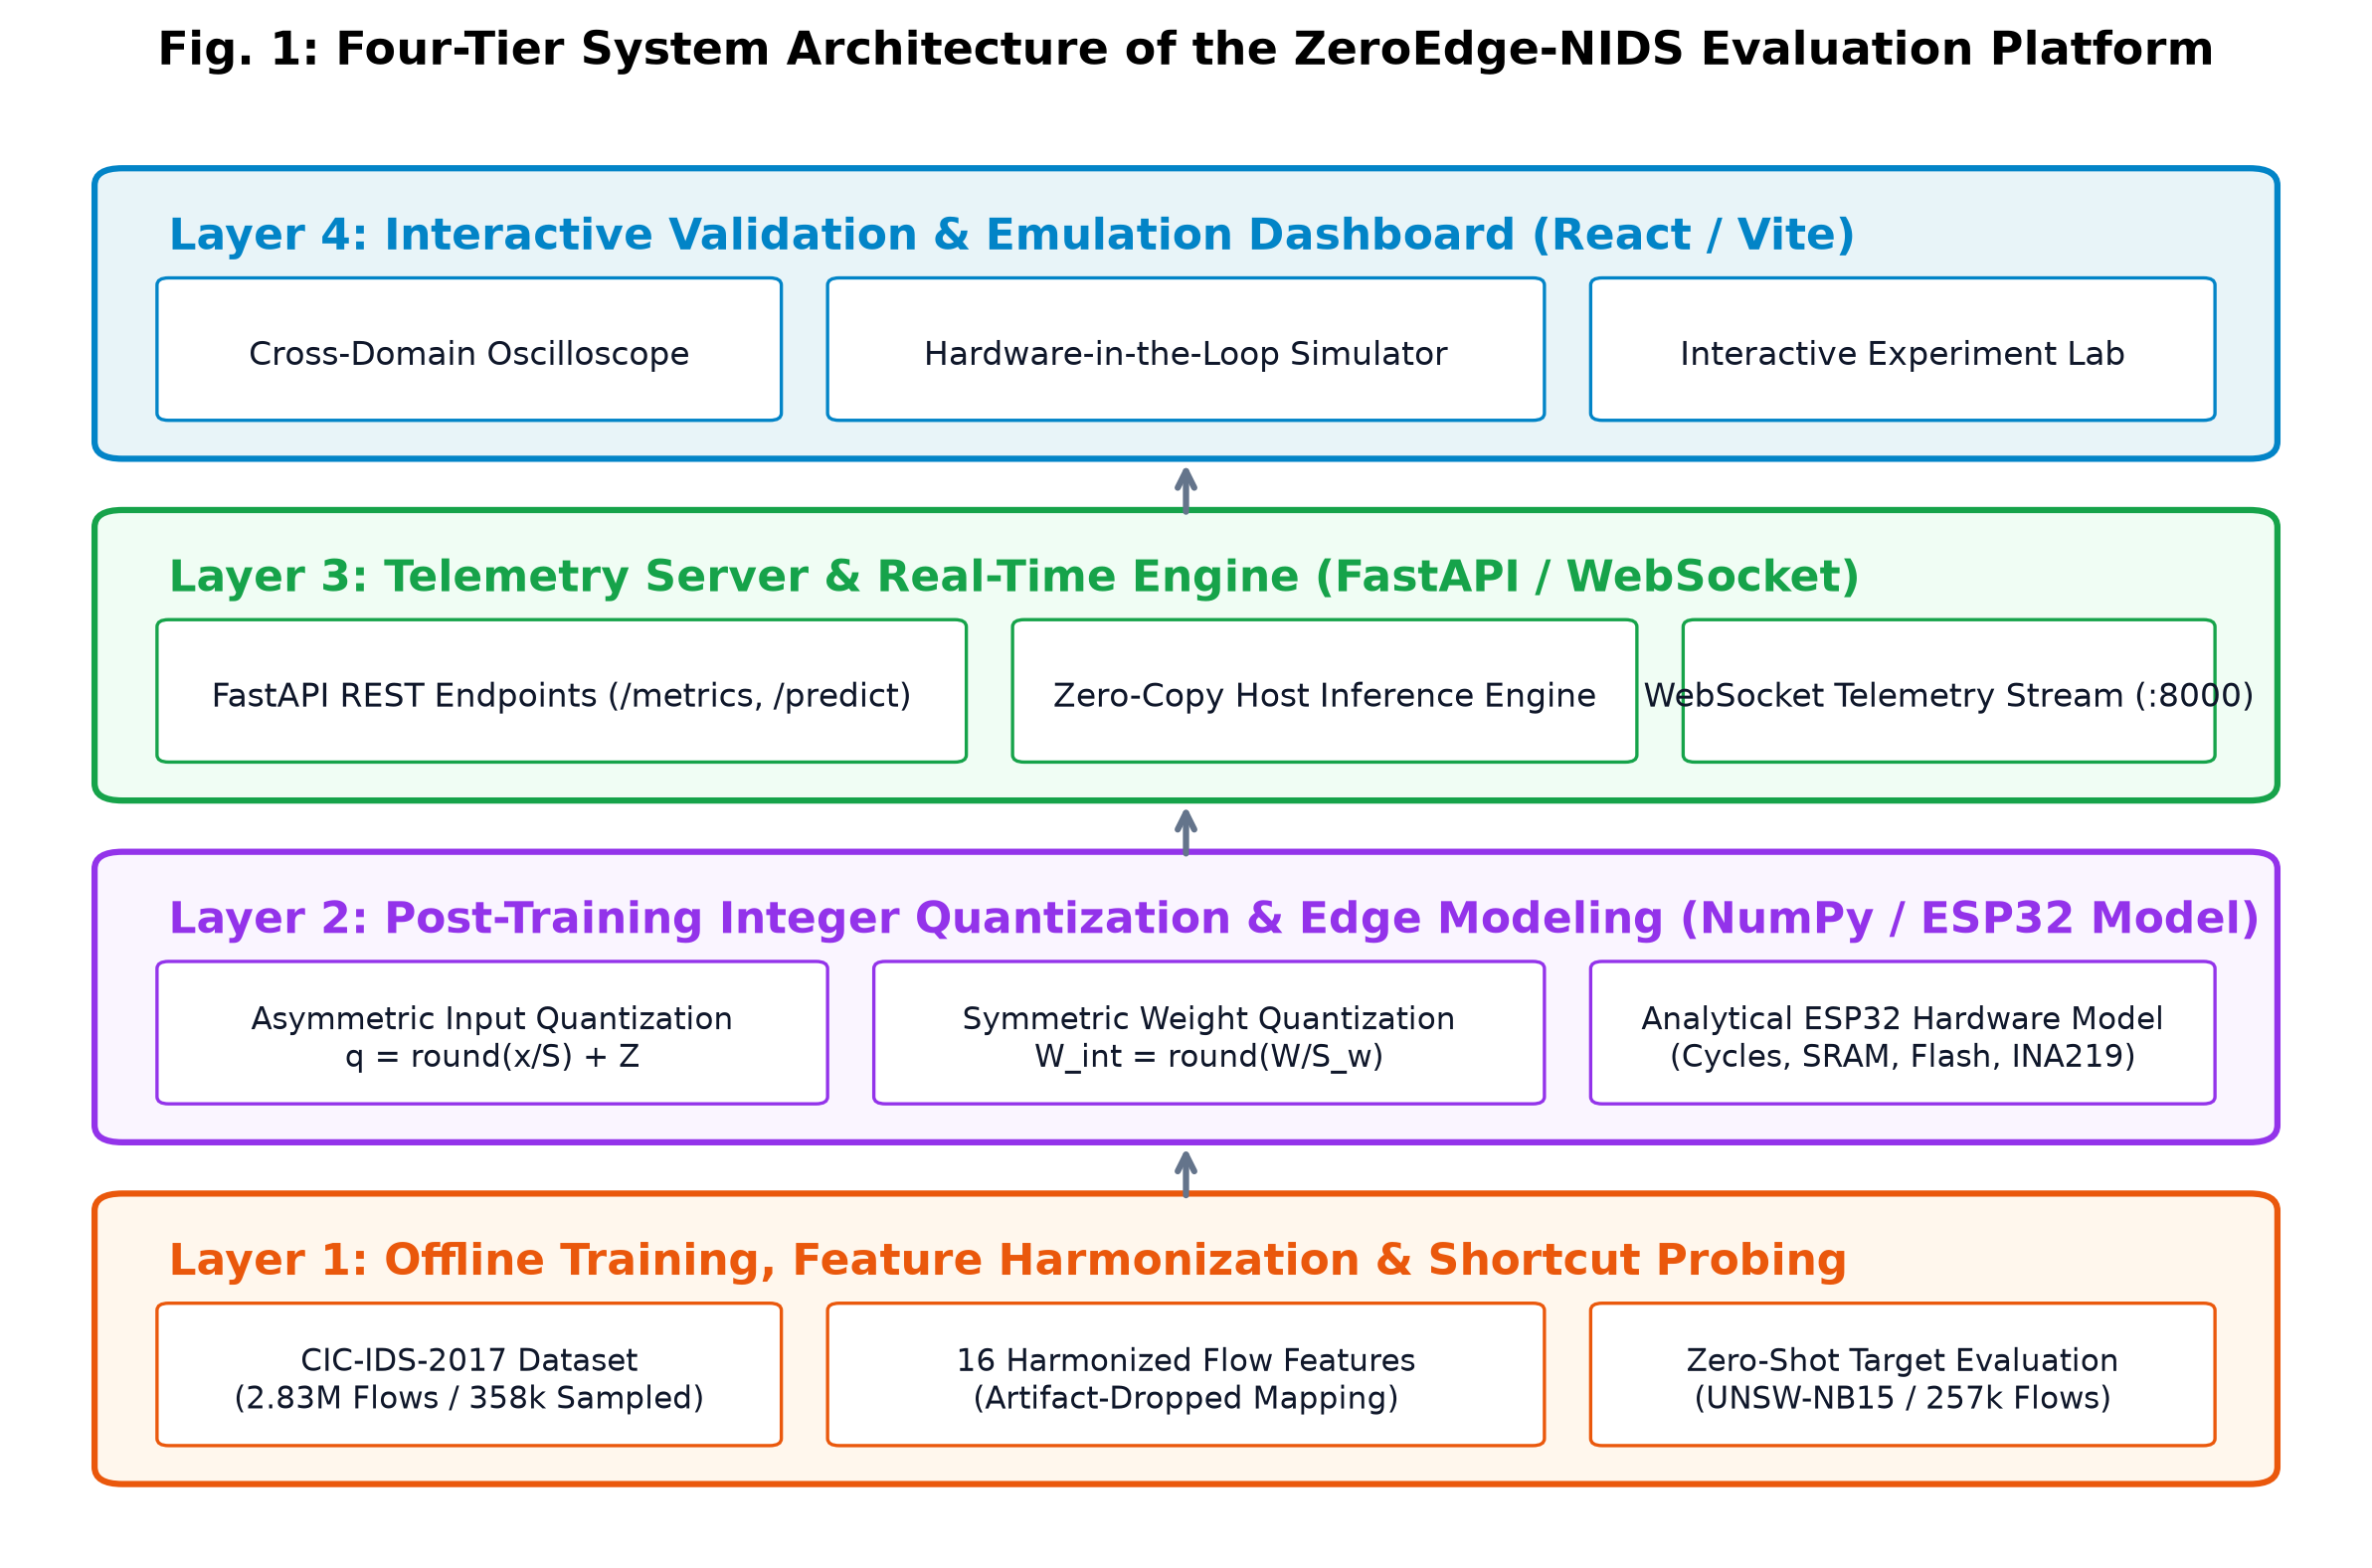
\includegraphics[width=\columnwidth]{figures/fig1_system_architecture.png}
\caption{Four-Tier System Architecture of the ZeroEdge-NIDS Evaluation Platform.}
\label{fig:arch}
\end{figure}

\begin{figure}[t]
\centering
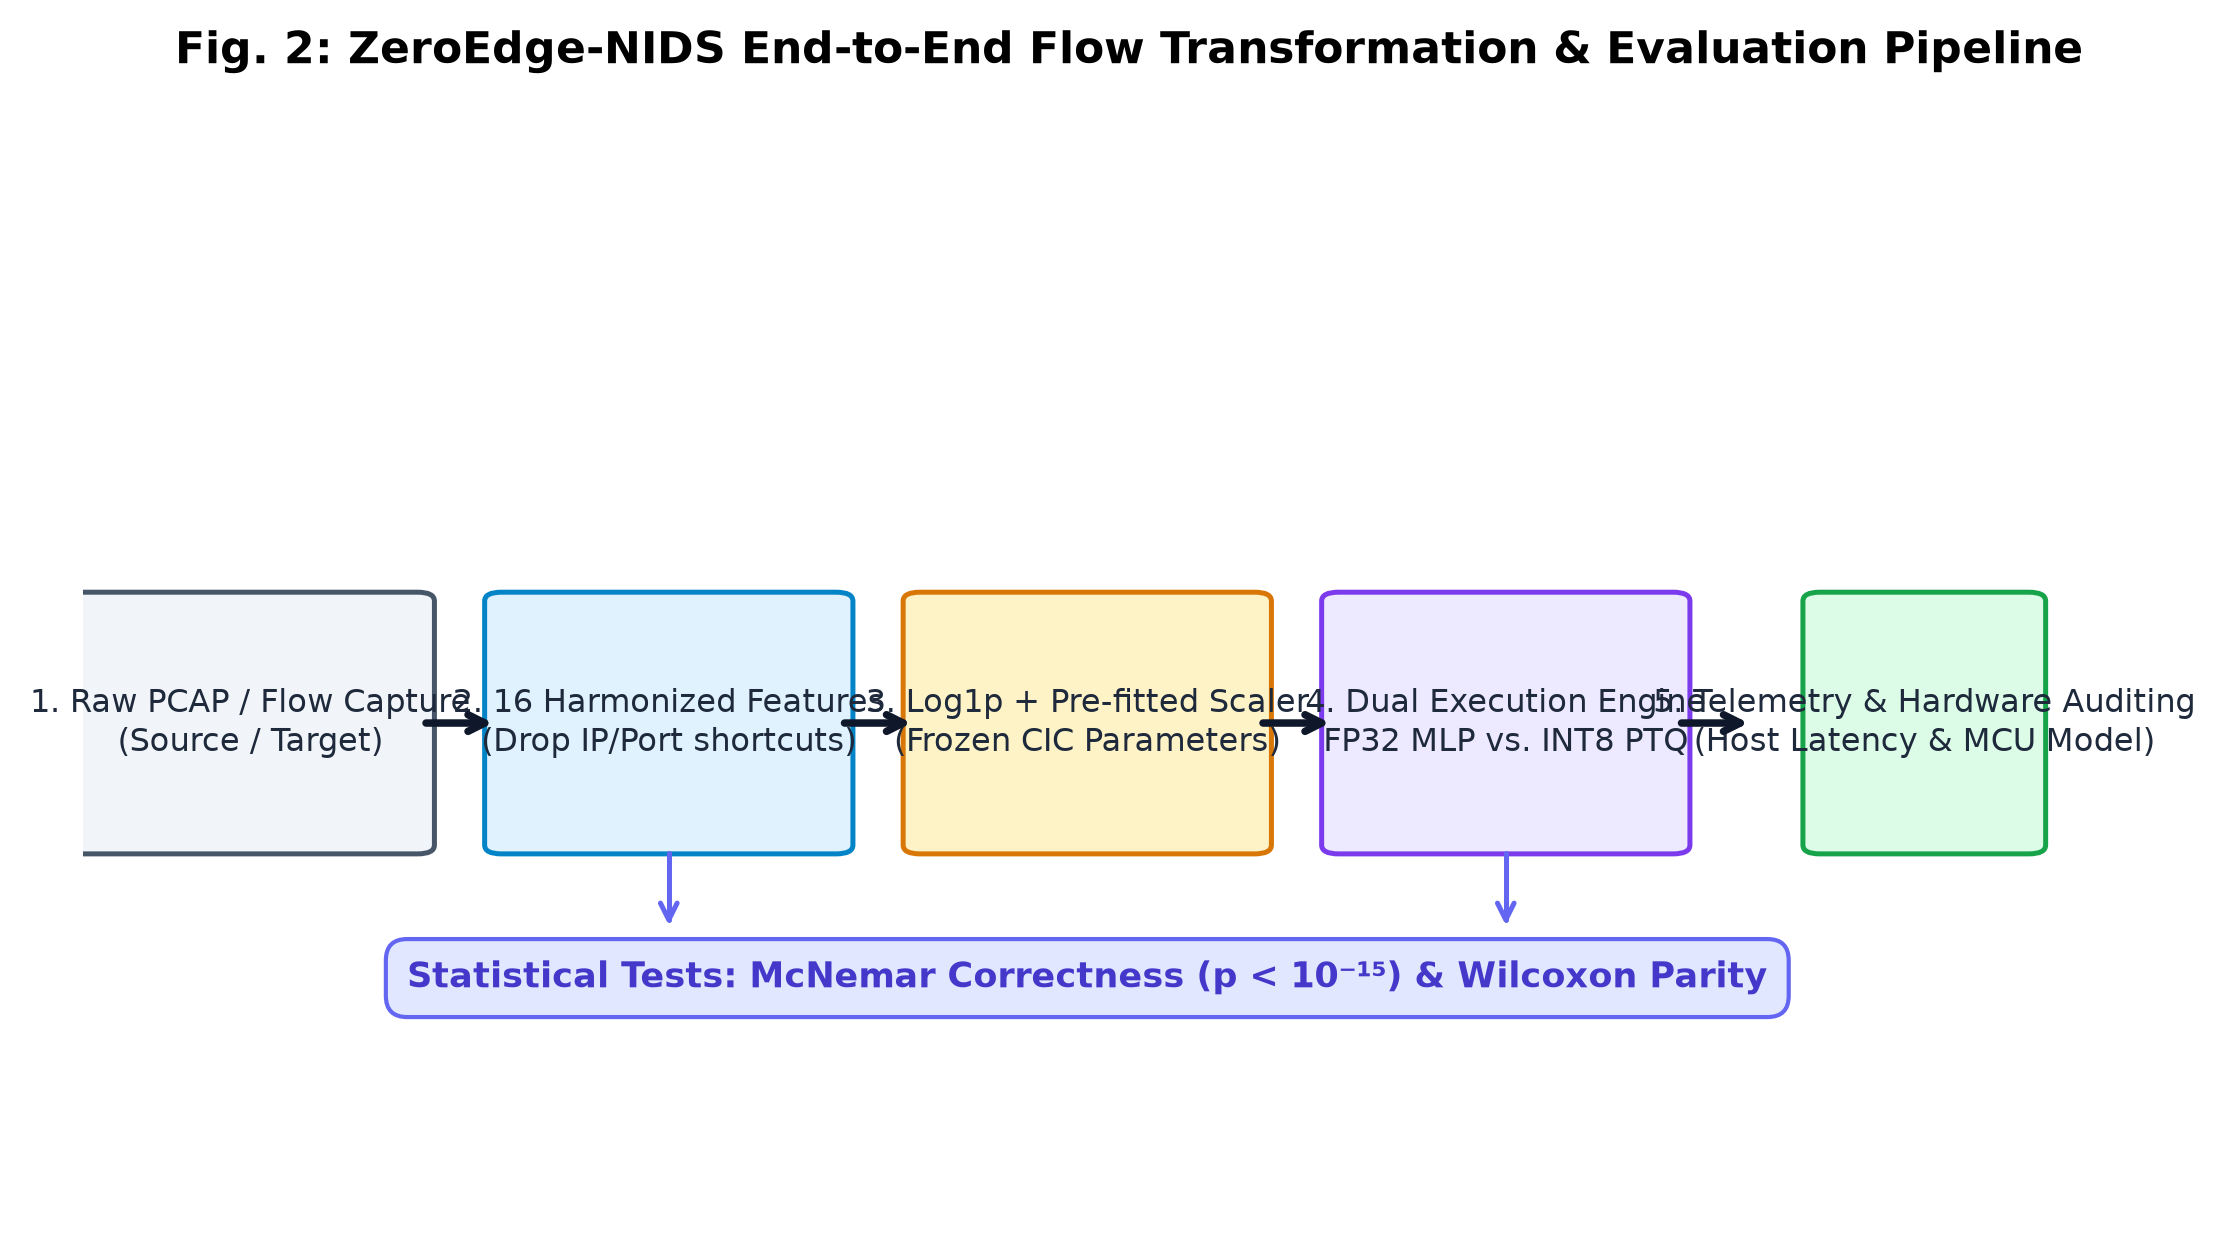
\includegraphics[width=\columnwidth]{figures/fig2_data_flow_sequence.png}
\caption{ZeroEdge-NIDS End-to-End Flow Transformation and Evaluation Pipeline.}
\label{fig:flow}
\end{figure}

\subsection{Canonical Feature Harmonization}
To facilitate zero-shot cross-domain evaluation between CIC-IDS-2017 and UNSW-NB15, we define a canonical 16-dimensional feature space $\mathbf{x} \in \mathbb{R}^{16}$. A central design requirement is the strict removal of explicit shortcut artifacts. We deliberately drop:
\begin{enumerate}
    \item \emph{Network and Transport Identifiers:} Source IP, Destination IP, Source Port, and Flow ID. (Destination Port is retained solely as an application protocol class proxy).
    \item \emph{Temporal Synchrony Artifacts:} Absolute packet timestamps and TCP window/sequence counters.
    \item \emph{Synthetic Capture Artifacts:} Inter-arrival jitter counters that reflect traffic generator clocks rather than intrinsic protocol behavior.
\end{enumerate}

The resulting 16 features capture pure aggregate statistical properties of bidirectional traffic flows:
\begin{itemize}
    \item Flow dynamics: \texttt{flow\_duration\_us}, \texttt{flow\_byts\_s}, \texttt{flow\_pkts\_s}.
    \item Packet volume: \texttt{total\_fwd\_packets}, \texttt{total\_bwd\_packets}, \texttt{total\_fwd\_bytes}, \texttt{total\_bwd\_bytes}.
    \item Packet length distributions: Forward packet lengths (\texttt{fwd\_pkt\_len\_max}, \texttt{fwd\_pkt\_len\_min}, \texttt{fwd\_pkt\_len\_mean}, \texttt{fwd\_pkt\_len\_std}) and backward packet lengths (\texttt{bwd\_pkt\_len\_max}, \texttt{bwd\_pkt\_len\_min}, \texttt{bwd\_pkt\_len\_mean}, \texttt{bwd\_pkt\_len\_std}).
    \item Port identifier: \texttt{dst\_port}.
\end{itemize}

\subsection{Feature Preprocessing & Frozen Min-Max Scaling}
Due to extreme heavy-tailed skewness common to network traffic volumes, logarithmic transformations are applied to heavily skewed attributes:
\begin{equation}
\tilde{x}_i = \ln(1 + x_i) \quad \text{for } i \in \mathcal{I}_{\text{skew}},
\end{equation}
where $\mathcal{I}_{\text{skew}}$ denotes features spanning multiple orders of magnitude (e.g., bytes, duration, packet rates).

To maintain absolute zero-shot evaluation integrity, normalization parameters are derived \emph{strictly from the CIC-IDS-2017 training partition}:
\begin{equation}
\hat{x}_i = \text{clip}\left(\frac{\tilde{x}_i - \min(X_{\text{train}, i})}{\max(X_{\text{train}, i}) - \min(X_{\text{train}, i})}, 0.0, 1.0\right).
\end{equation}
Critically, these min-max bounds are \emph{never updated or refit} on the UNSW-NB15 target evaluation set. Values falling outside the training distribution are clipped to $[0.0, 1.0]$, and logged as out-of-bounds drift observations.

\subsection{Baseline Neural Network Architecture}
The baseline classifier is a compact Multi-Layer Perceptron (MLP) optimized for microcontrollers:
\begin{equation}
\mathbf{h}_1 = \text{ReLU}(\mathbf{W}_1 \hat{\mathbf{x}} + \mathbf{b}_1) \in \mathbb{R}^{32},
\end{equation}
\begin{equation}
\mathbf{h}_2 = \text{ReLU}(\mathbf{W}_2 \mathbf{h}_1 + \mathbf{b}_2) \in \mathbb{R}^{16},
\end{equation}
\begin{equation}
\hat{y} = \sigma(\mathbf{W}_3 \mathbf{h}_2 + b_3) \in [0, 1],
\end{equation}
where $\sigma(z) = 1 / (1 + e^{-z})$, and $\mathbf{W}_1 \in \mathbb{R}^{32 \times 16}$, $\mathbf{W}_2 \in \mathbb{R}^{16 \times 32}$, $\mathbf{W}_3 \in \mathbb{R}^{1 \times 16}$. The network comprises exactly $1,040$ weights, $49$ biases ($1,089$ total parameters), and executes $1,040$ multiply-accumulate operations per inference. Classification decisions use a standard threshold $\tau = 0.5$:
\begin{equation}
\hat{c} = \mathbb{I}(\hat{y} \ge 0.5).
\end{equation}

\subsection{Integer-Only Quantization Formulation}
We implement uniform affine Post-Training Quantization (PTQ) conforming to the integer-arithmetic paradigm of Jacob et al.~\cite{jacob2018quantization}. A real-valued continuous tensor $r \in \mathbb{R}$ is approximated by an 8-bit quantized integer $q \in [\alpha, \beta]$ via:
\begin{equation}
r \approx S \cdot (q - Z),
\label{eq:quant}
\end{equation}
where $S \in \mathbb{R}^+$ is an arbitrary positive real scaling factor and $Z \in \mathbb{Z}$ is the zero-point offset ensuring that real zero maps exactly to an integer.

\subsubsection{Asymmetric Input Quantization}
Because normalized input vectors satisfy $\hat{\mathbf{x}} \in [0.0, 1.0]$, asymmetric quantization maps the range $[0, 1]$ into signed 8-bit integers $q \in [-128, 127]$:
\begin{equation}
S_{\text{in}} = \frac{r_{\max} - r_{\min}}{q_{\max} - q_{\min}} = \frac{1.0 - 0.0}{127 - (-128)} = \frac{1.0}{255} \approx 0.00392157,
\end{equation}
\begin{equation}
Z_{\text{in}} = \text{round}\left(- \frac{r_{\min}}{S_{\text{in}}}\right) + q_{\min} = 0 + (-128) = -128,
\end{equation}
\begin{equation}
\mathbf{q}_{\text{in}} = \text{clip}\left(\text{round}\left(\frac{\hat{\mathbf{x}}}{S_{\text{in}}}\right) + Z_{\text{in}}, -128, 127\right).
\end{equation}

\subsubsection{Symmetric Weight Quantization}
Weight tensors $\mathbf{W}_l$ are quantized symmetrically with zero-point $Z_W = 0$ to eliminate zero-point cross-terms in matrix multiplication:
\begin{equation}
S_{W, l} = \frac{\max(|\min(\mathbf{W}_l)|, |\max(\mathbf{W}_l)|)}{127},
\end{equation}
\begin{equation}
\mathbf{Q}_{W, l} = \text{clip}\left(\text{round}\left(\frac{\mathbf{W}_l}{S_{W, l}}\right), -128, 127\right).
\end{equation}

\subsubsection{Integer-Only Forward Propagation}
Substituting Eq.~\eqref{eq:quant} into linear transformation $r_{\text{out}} = \mathbf{W} r_{\text{in}} + b$ yields:
\begin{equation}
S_{\text{out}}(q_{\text{out}} - Z_{\text{out}}) = \sum_{j} S_W Q_{W, j} \cdot S_{\text{in}} (q_{\text{in}, j} - Z_{\text{in}}) + b.
\end{equation}
Defining the effective real multiplier $M = \frac{S_{\text{in}} S_W}{S_{\text{out}}}$:
\begin{equation}
q_{\text{out}} = Z_{\text{out}} + \text{round}\left( M \left[ \sum_{j} Q_{W, j}(q_{\text{in}, j} - Z_{\text{in}}) + \frac{b}{S_{\text{in}} S_W} \right] \right).
\label{eq:int_eval}
\end{equation}
The inner summation $\sum_{j} Q_{W, j}(q_{\text{in}, j} - Z_{\text{in}})$ accumulates into a 32-bit signed integer ($\text{INT32}$) accumulator, preventing overflow. On microcontrollers lacking floating-point hardware, $M \in (0, 1)$ is decomposed into a fixed-point mantissa $M_0 \in [2^{30}, 2^{31})$ and a right bit-shift $n$:
\begin{equation}
M \approx 2^{-n} M_0.
\end{equation}

\subsection{Analytical ESP32 Hardware Modeling}
To quantify deployment feasibility without relying on ungrounded hardware claims, we implement an analytical hardware model parameterized for the Espressif ESP32 (Xtensa LX6 dual-core Harvard architecture operating at $240\ \text{MHz}$, clock period $T_{\text{clk}} = 4.167\ \text{ns}$).
\begin{itemize}
    \item \textbf{Cycle Accounting:} The Xtensa LX6 provides single-cycle 32-bit integer MAC instructions (\texttt{MUL16}, \texttt{ADD}), whereas software-emulated or single-precision FP32 MAC operations require approximately $16\text{--}24$ cycles including load/store pipelining. Total execution cycles are modeled as:
    \begin{equation}
    C_{\text{INT8}} = N_{\text{MAC}} \cdot c_{\text{MAC, INT8}} + N_{\text{act}} \cdot c_{\text{act}} + C_{\text{ovh}},
    \end{equation}
    yielding $C_{\text{INT8}} = 5,504$ cycles ($22.93\ \mu\text{s}$) versus $C_{\text{FP32}} = 19,920$ cycles ($83.00\ \mu\text{s}$).
    \item \textbf{Tensor Arena SRAM:} In TinyML execution graphs, activation buffers are multiplexed across sequential layers. Memory footprint is strictly bounded by the maximum adjacent layer activation tensors:
    \begin{equation}
    \text{SRAM}_{\text{arena}} = \max_l (A_l + A_{l+1}) + \text{TFLM overhead}.
    \end{equation}
    For our architecture, INT8 requires $4,160$ bytes ($1.27\%$ of the 320 KB usable SRAM), compared to $4,304$ bytes for FP32.
    \item \textbf{Flash Footprint:} Flash utilization is dominated by serialized model parameters. INT8 stores weights as signed 8-bit integers ($1,040$ bytes) plus quantized biases and scaling constants, occupying $1,236$ bytes ($0.029\%$ of 4 MB flash)—a $71.63\%$ reduction relative to FP32 ($4,356$ bytes).
    \item \textbf{Energy & Power Consumption:} Modeled after a Texas Instruments INA219 current sensor monitoring a $3.3\ \text{V}$ supply rail:
    \begin{equation}
    E_{\text{inf}} = V_{\text{dd}} \cdot I_{\text{active}} \cdot t_{\text{latency}} = 3.3\ \text{V} \times 62.0\ \text{mA} \times 22.93\ \mu\text{s} = 4.69\ \mu\text{J}.
    \end{equation}
\end{itemize}
